\documentclass[12pt]{article}

%%%%%%%%%%%%%%%%%%%%%%%%%%%%%%%%%%%%%%%%%%%%%%%%%%%%%%%%%%%%%%%%%%%%%%%%
%% Customizações do abnTeX2 (http://abnTeX2.googlecode.com)           %%
%% para a Universidade Estadual do Ceara - UECE                       %%
%%                                                                    %%
%% This work may be distributed and/or modified under the             %%
%% conditions of the LaTeX Project Public License, either version 1.3 %%
%% of this license or (at your option) any later version.             %%
%% The latest version of this license is in                           %%
%%   http://www.latex-project.org/lppl.txt                            %%
%% and version 1.3 or later is part of all distributions of LaTeX     %%
%% version 2005/12/01 or later.                                       %%
%%                                                                    %%
%% This work has the LPPL maintenance status `maintained'.            %%
%%                                                                    %%
%% The Current Maintainer of this work is Thiago Nascimento           %%
%%                                                                    %%
%% Project available on: https://github.com/thiagodnf/uecetex2        %%
%%                                                                    %%
%% Further information about abnTeX2                                  %%
%% are available on http://abntex2.googlecode.com/                    %%
%%                                                                    %%
%%%%%%%%%%%%%%%%%%%%%%%%%%%%%%%%%%%%%%%%%%%%%%%%%%%%%%%%%%%%%%%%%%%%%%%%

% \documentclass[
%     a4paper,          % Tamanho da folha A4
%     12pt,             % Tamanho da fonte 12pt
%     chapter=TITLE,    % Todos os capitulos devem ter caixa alta
%     section=TITLE,    % Todas as secoes devem ter caixa alta
%     oneside,          % Usada para impressao em apenas uma face do papel
%     english,          % Hifenizacoes em ingles
%     spanish,          % Hifenizacoes em espanhol
%     brazil            % Ultimo idioma eh o idioma padrao do documento
% ]{abntex2}



% Importações de pacotes
\usepackage[utf8]{inputenc}                         % Acentuação direta
\usepackage[T1]{fontenc}                            % Codificação da fonte em 8 bits
\usepackage{graphicx}                               % Inserir figuras
\usepackage{amsfonts, amssymb, amsmath}             % Fonte e símbolos matemáticos
\usepackage{booktabs}                               % Comandos para tabelas
\usepackage{verbatim}                               % Texto é interpretado como escrito no documento
\usepackage{multirow, array}                        % Múltiplas linhas e colunas em tabelas
\usepackage{indentfirst}                            % Endenta o primeiro parágrafo de cada seção.
\usepackage{listings}                               % Utilizar codigo fonte no documento
\usepackage{xcolor}
\usepackage{microtype}                              % Para melhorias de justificação?
\usepackage[portuguese,ruled,lined]{algorithm2e}    % Escrever algoritmos
\usepackage{algorithmic}                            % Criar Algoritmos
\usepackage{float}                                  % Utilizado para criação de floats
\usepackage{amsgen}
\usepackage{lipsum}                                 % Usar a simulação de texto Lorem Ipsum
%\usepackage{titlesec}                               % Permite alterar os títulos do documento
\usepackage{tocloft}                                % Permite alterar a formatação do Sumário
\usepackage{etoolbox}                               % Usado para alterar a fonte da Section no Sumário
\usepackage[nogroupskip,nonumberlist,acronym]{glossaries}                % Permite fazer o glossario
\usepackage{caption}                                % Altera o comportamento da tag caption
\usepackage[num, abnt-emphasize=bf, bibjustif, recuo=0cm, abnt-etal-cite=2, abnt-etal-list=0]{abntex2cite}  % Citações padrão ABNT
%\usepackage[bottom]{footmisc}                      % Mantém as notas de rodapé sempre na mesma posição
%\usepackage{times}                                 % Usa a fonte Times
\usepackage{mathptmx}                               % Usa a fonte Times New Roman
%\usepackage{lmodern}                               % Usa a fonte Latin Modern
%\usepackage{subfig}                                % Posicionamento de figuras
%\usepackage{scalefnt}                              % Permite redimensionar tamanho da fonte
%\usepackage{color, colortbl}                        % Comandos de cores
%\usepackage{lscape}                                % Permite páginas em modo "paisagem"
%\usepackage{ae, aecompl}                           % Fontes de alta qualidade
%\usepackage{picinpar}                              % Dispor imagens em parágrafos
%\usepackage{latexsym}                              % Símbolos matemáticos
%\usepackage{upgreek}                               % Fonte letras gregas
\usepackage{appendix}                               % Gerar o apendice no final do documento
\usepackage{paracol}                                % Criar paragrafos sem identacao
\usepackage{lib/uecetex2}		                    % Biblioteca com as normas da UECE para trabalhos academicos
\usepackage{pdfpages}                               % Incluir pdf no documento
\usepackage{amsmath}                                % Usar equacoes matematicas

\usepackage{hyperref}

\usepackage{glossaries}

\usepackage{enumerate}
\usepackage{enumitem}

\renewcommand{\ABNTEXchapterfontsize}{\normalsize}

\renewcommand{\ABNTEXsectionfontsize}{\normalsize}

% Organiza e gera a lista de abreviaturas, simbolos e glossario
\makenoidxglossaries

% Gera o Indice do documento
\makeindex


\sloppy

\title{Uma Revisão de Literatura sobre \textit{Ferramentas Computacionais para
        o Estudo da Evolução de Espécies Baseado no Uso de Códons}}

\author{Mauricio Souza Menezes Teste\\}
\address{Departamento de Ciências Exatas e da Terra, Campus I\\
    Universidade do Estado da Bahia (UNEB)\\
    Salvador, Bahia, Brasil.
    \email{mauriciosm95@gmail.com}
}

\begin{document}

\newacronym{ufm}{UFM}{Universal Feature Method}
\newacronym{ngs}{NGS}{Sequenciamento de Nova Geração}
\newacronym{rs}{RS}{Revisão Sistemática}
\newacronym{cafe}{CAFe}{Comunidade Acadêmica Federada}
\newacronym{parsifal}{Parsifal}{Perform Systematic Literature Reviews}
\newacronym{fcgr}{FCGR}{Frequency Chaos Game Representation}

\maketitle

\begin{resumo}
    Esta \gls{rs} dos métodos de classificação genética de sequências implementados e aplicados até o momento. Vários métodos diferentes foram identificados, sugerindo que nenhum deles foi considerado indubitável.
\end{resumo}

\begin{abstract}
    \begin{otherlanguage}{english}
        This Systematic Review (SR) of sequence genetic classification methods implemented and applied to date. Several different methods were identified, suggesting that none of them was considered indubitable.
    \end{otherlanguage}
\end{abstract}

\section{Introdução}

As análises de reconstrução filogenética é uma ferramenta muito utilizada no campo das Ciências Biológicas. O seu uso busca identificar e compreender as relações evolutivas entre diferentes formas de vida no planeta, pois ela busca compreender a evolução de agentes causadores de doenças.
Segundo~\cite{behl_threat_2022} `existe uma tendência histórica, onde os vírus e bactérias sofrem mutações no decorrer do tempo, encontrando mecanismos para infectar as células humanas.'
Este artigo apresenta uma \gls{rs} da literatura referente aos métodos computacionais utilizados para realizar o estudo de especiação genômica. Os artigos foram obtidos através da busca realizada em quatro bases de dados (PubMed, ScienceDirect, Scopus e Springer Link) levando em conta a principal questão: Quais métodos são utilizados para realizar o estudo de especiação? Foram incluídos todos os artigos que atenderam aos critérios definidos.

\section{Relato da Revisão de Literatura}

Logo após definir os objetivos da pesquisa, foi primordial conhecer os pormenores que estavam relacionados aos mesmos, e para isso foi necessário realizar uma \gls{rs}. Dessa forma, foi utilizado um protocolo que serviria de base no processo para a obtenção dos estudos que deveriam ser analisados, os quais foram definidos e analisados através de: Objetivos, questões, palavras-chave, strings de busca, fontes e critérios para inclusão e exclusão.

\subsection{Objetivo da Pesquisa}

A pesquisa teve como objetivo verificar e conhecer a existência de métodos utilizados para a analise da evolução de espécies com base no uso de códons, a identificação do que já foi feito para sanar o problema identificado e também se era viável ou não o desenvolvimento de uma nova solução para classificação gênica.

\subsection{Questões de Pesquisa}

Foram definidas duas questões de pesquisa. A primeira e principal questionava quais métodos são utilizados para realizar o estudo de especiação. Enquanto a segunda era se alguma dessas metodologias é baseada no uso/frequência de códons. As questões de pesquisa foram escolhidas com base naquilo que se queria entender ao final da \gls{rs}.

\subsection{Repositório de Busca de Dados}

As bases precisavam conter trabalhos relevantes relacionados a bioinformática, completos e gratuitos. No entanto, em alguns casos, esse acesso se deu através por meio do portal da \gls{cafe}. Deste modo, as seguintes bases de dados acadêmicos foram selecionadas:
\begin{itemize}
    \item{PubMed}
    \item{ScienceDirect}
    \item{Scopus}
    \item{Springer Link}
\end{itemize}

Para o refinamento das consultas foram utilizados os filtros que serão apresentados a seguir:

\begin{enumerate}
    \item ScienceDirect
          \begin{enumerate}
              \item Article type: Review Articles e Research Articles
              \item Access type: Open access e Open Archive
              \item Years: 2018 até 2022
          \end{enumerate}
    \item Springer Link
          \begin{enumerate}
              \item Include preview-only content: Desmarcado
              \item Content type: Article
              \item Language: English
              \item Years: 2018 até 2022
          \end{enumerate}
    \item Scopus
          \begin{enumerate}
              \item Open access: All open access
              \item Years: 2018 até 2022
          \end{enumerate}
\end{enumerate}


\subsection{Palavras-chave e Strings de Busca}

As palavras-chave, com seus sinônimos e correlatos em inglês, selecionadas para a busca nas bases de dados, com o objetivo de encontrar o máximo de estudos relevantes, foram as seguintes:
\begin{itemize}
    \item{Bioinformatics e Bioinformática}
    \item{Codon e códon}
    \item{Gene}
    \item{Phylogeny e filogenia}
    \item{Classification, classificação, genotyping, genotipagem, subtyping, subtipagem, typing e tipagem}
    \item{Viral}
\end{itemize}
Com base nas palavras-chave, foi criada a string de busca a seguir, que foi utilizada em todas as bases de dados.

\begin{itemize}
    \item ((`bioinformatics') AND (`codon') AND (`phylogeny') AND (`typing' OR `classification' OR `genotyping' OR `subtyping') AND (`gene') AND (`viral'))
\end{itemize}

\subsection{Critérios de seleção}

Para realizar o processo de seleção dos estudos foram definidos critérios, podendo ser de inclusão ou de exclusão.
Os critérios de inclusão foram os seguintes:

\begin{itemize}
    \item I1: O estudo contém as palavras-chave definidas na pesquisa no resumo, título ou palavras-chave.
    \item I2: Aborda algum método de especiação.
\end{itemize}
Os critérios de exclusão foram os seguintes:
\begin{itemize}
    \item E1: O tema do estudo não está relacionado à especiação.
    \item E2: O tema do estudo não é pertinente com a área/objetivos da pesquisa.
    \item E3: O estudo está duplicado.
\end{itemize}

\section{Resultados Parciais}

\subsection{Análise Quantitativa dos Resultados}

A aplicação das strings nas bases de dados selecionadas, resultou em um total geral de 177 (cento e setenta e sete) artigos, os quais foram oriundos da fonte PubMed 3 (três) artigos, da fonte ScienceDirect 85 (oitenta e cinco) artigos, da fonte Scopus 10 (dez) artigos e da fonte Springer Link 79 (setenta e nove) artigos.\\
Após o processo de obtenção, foi iniciada a seleção dos artigos, onde foi realizada a leitura do título, resumo e palavras-chave, aplicando os critérios de inclusão e exclusão. Esse processo resultou em: 26 (vinte e seis) artigos aceitos; 147 (cento e quarenta e sete) artigos rejeitados; e 4 (quatro) artigos duplicados. Os resultados são apresentados nos gráficos nas figuras~\ref{fig:artigoBases} e~\ref{fig:excluidosCriterios}.\\


\begin{figure}[tb]
    \centering
    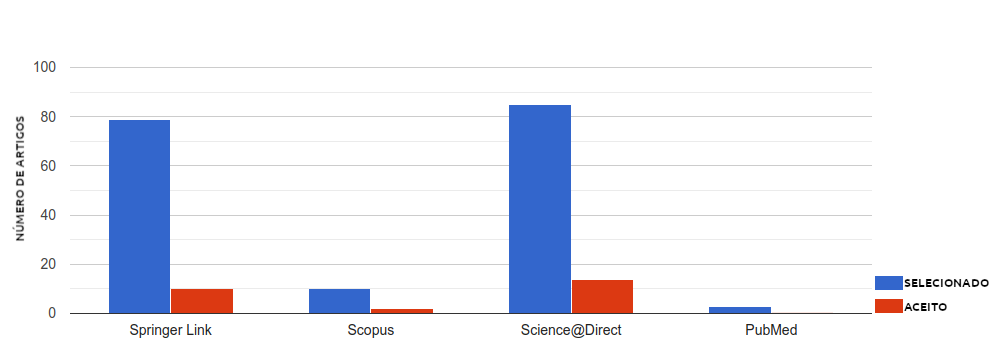
\includegraphics[scale=0.42]{figuras/_artigosAceitosSelecionados.png}
    \caption{Artigos Selecionados e Aceitos por Base.}\label{fig:artigoBases}
\end{figure}

\begin{figure}[tb]
    \centering
    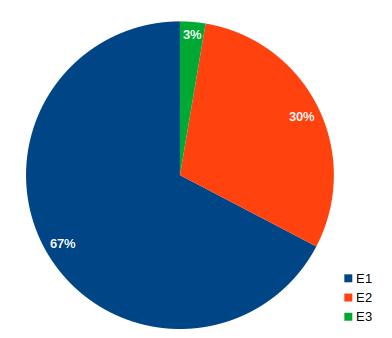
\includegraphics[scale=0.5]{figuras/_artigosExcluidosPorCriterio.png}
    \caption{Artigos Excluídos por Critério.}\label{fig:excluidosCriterios}
\end{figure}


\subsection{Análise Qualitativa dos Resultados}

Na etapa de extração, realizada com o auxílio da ferramenta \gls{parsifal}, houve o levantamento de informações para ajudar a responder as questões de pesquisa, 4(quatro) para a principal e 1(uma) para a secundaria, apresentadas a seguir: \\

\begin{itemize}
    \item P1: Qual método de classificação genética foi utilizado?
    \item P2: O método necessitava de algum treinamento?
    \item P3: Se necessita de algum treinamento, o mesmo era supervisionado?
    \item P4: O método necessitava de uma árvore de referência supervisionada?
    \item S1: Alguma dessas metodologias é baseada no uso/frequência de códons?
\end{itemize}

Essas informações foram importantes também para a construção da planilha-resumo de resultados. Também é importante salientar, que após a leitura completa, 12(doze) dos trabalhos se enquadraram em um dos critérios de exclusão apresentados anteriormente.

Se tratando dos métodos de classificação gênica utilizados, o trabalho~\cite{dimitrov_updated_2019} apresentou e comparou três modelos para reconstrução de árvores filogenéticas: junção de vizinhos; máxima verossimilhança e inferência bayesiana.
Para ~\cite{yin_systematic_2019} e ~\cite{bedoya-pilozo_molecular_epidemiology_2018} foi usada a inferência bayesiana. Temos que em ~\cite{fall_genetic_diversity_2021},~\cite{behl_threat_2022},~\cite{shabbir_comprehensive_2020}, ~\cite{hudu_hepatitis_2018}, ~\cite{sallard_tracing_2021},~\cite{paez-espino_diversity_evolution_2019}, ~\cite{tang_evolutionary_2021} e ~\cite{cho_analysis_2022} foi aplicada a máxima verossimilhança.
Os demais estudos apresentaram metodologias distintas: No trabalho de ~\cite{lichtblau_alignment-free_2019} foi \gls{fcgr}; ~\cite{kim_ngs_2022} a floresta aleatória e ~\cite{potdar_phylogenetic_2021} a junção de vizinhos.
Além disso, levando em conta a necessidade de treinamento, ~\cite{lichtblau_alignment-free_2019} utilizou redes neurais, onde não houve treinamento supervisionado ou necessidade de uma árvore de referência supervisionada.

Já em relação metodologias baseadas em uso/frequência de códons, nenhum dos trabalhos apresentou tal proposta. O que mais se aproximou disso foi~\cite{cho_analysis_2022} que segundo ele `realizou um agrupamento da análise do uso de códons com base nos resultados das árvores filogenéticas'.

\section{Conclusões}

A possibilidade do desenvolvimento de uma ferramenta de classificação gênica com base no uso/frequência de códons se mostrou possível, tendo em vista que os métodos encontrados não realizavam tal metodologia. Sendo assim, uma nova sistematização para classificação de sequências genéticas poderá contribuir com avanços na otimização de classificação de grandes conjuntos de dados para determinar a sua caracterização genômica.

\bibliographystyle{sbc}
\bibliography{RefGeral}

\pagebreak
\begin{landscape}

    \section{Planilha-resumo de Resultados}

    Na~\ref{tab:resumo} é apresentada a planilha-resumo de resultados com os trabalhos aceitos no processo de seleção. Assim, para cada artigo foi extraído a sua identificação, os critérios de inclusão ou exclusão que foram aplicados, uma breve descrição e as respostas para as perguntas apresentadas na seção de análise qualitativa dos resultados. Alguns campos foram respondidos com S (sim), N (não) e O (Omitido).

    \begin{center}

        \begin{longtable}{p{8cm}|c|c|c|c|c|p{5cm}|p{3cm}|c|c|c|c}
            \caption{Planilha-resumo dos trabalhos selecionados.}\label{tab:resumo}
            \\
            \multicolumn{1}{c|}{\textbf{Identificação do Trabalho}} &
            \multicolumn{1}{c|}{\textbf{I1}}                        &
            \multicolumn{1}{c|}{\textbf{I2}}                        &
            \multicolumn{1}{c|}{\textbf{E1}}                        &
            \multicolumn{1}{c|}{\textbf{E2}}                        &
            \multicolumn{1}{c|}{\textbf{E3}}                        &
            \multicolumn{1}{c|}{\textbf{Descrição}}                 &
            \multicolumn{1}{c|}{\textbf{P1}}                        &
            \multicolumn{1}{c|}{\textbf{P2}}                        &
            \multicolumn{1}{c|}{\textbf{P3}}                        &
            \multicolumn{1}{c|}{\textbf{P4}}                        &
            \multicolumn{1}{c}{\textbf{S1}}

            \\ \hline
            \hline
            \endfirsthead

            \multicolumn{8}{c}%
            {{\bfseries \tablename\ \thetable{} -- continuação da página
                        anterior}}

            \\
            \multicolumn{1}{c|}{\textbf{Identificação do Trabalho}} &
            \multicolumn{1}{c|}{\textbf{I1}}                        &
            \multicolumn{1}{c|}{\textbf{I2}}                        &
            \multicolumn{1}{c|}{\textbf{E1}}                        &
            \multicolumn{1}{c|}{\textbf{E2}}                        &
            \multicolumn{1}{c|}{\textbf{E3}}                        &
            \multicolumn{1}{c|}{\textbf{Descrição}}                 &
            \multicolumn{1}{c|}{\textbf{P1}}                        &
            \multicolumn{1}{c|}{\textbf{P2}}                        &
            \multicolumn{1}{c|}{\textbf{P3}}                        &
            \multicolumn{1}{c|}{\textbf{P4}}                        &
            \multicolumn{1}{c}{\textbf{S1}}

            \\ \hline
            \hline
            \endhead

            \hline \multicolumn{8}{r}{{Continua na próxima página}}

            \\
            \endfoot
            \hline \hline
            \endlastfoot

            \bibentry{ahmad_comprehensive_2022}                     &
                                                                    & X &  &  &  & O estudo tem como objetivo investigar e analisar a mutação d 157 genomas de SARS-Cov-2 e suas variantes Delta e Omicron.                                                                                                            & Neighbor-Joining&N&N&N&N                                                                  \\
            \hline
            \bibentry{yin_systematic_2019}                          &
                                                                    & X &  &  &  & O estudo apresentou a reconstrução a filogenia do HBV com base em 4.429 sequências completas.                                                                                                                                       & Inferência bayesiana&N&N&N&N                                                                                                                                                \\
            \hline
            \bibentry{lichtblau_alignment-free_2019}                &
                                                                    & X &  &  &  & O estudo apresentou a utilização de métodos livres de alinhamento de comparação genômica para escalonamento de grandes conjuntos de dados de sequências de nucleotídeos.                                                            & Frequency Chaos Game Representation (FCGR).&S&N&O&N                                        \\
            \hline
            \bibentry{cho_analysis_2022}                            &
            X                                                       & X &  &  &  & O estudo teve como objetivo confirmar o padrão geral de uso de códons e explorar as características evolutivas e genéticas comumente ou especificamente expressas em HIV1, HIV2 e SIV.                                              & Máxima verossimilhança&N&O&O&S                              \\
            \hline
            \bibentry{paez-espino_diversity_evolution_2019}                   &
                                                                    & X &  &  &  & O trabalho examinou uma coleção com 14.000 metagenomas, identificando 44.221 sequências de virófagos, das quais 328 era genomas completos ou quase completos. Nesses foi realizada a analise genômica comparativa.                  & Alinhamento concatenado.&N&N&N&N                                                                                                               \\
            \hline
            \bibentry{tang_evolutionary_2021}                       &
                                                                    & X &  &  &  & O estudo analisou variantes de nucleotídeo único (SNVs) em 121.618 genomas de SARS-CoV-2 de alta qualidade.                                                                                                                         & Máxima parcimônia&N&N&N&N                                                                                                                   \\
            \hline
            \bibentry{fall_genetic_diversity_2021}                            &
                                                                    & X &  &  &  & O estudo analisou a diversidade genética e a dinâmica evolutiva do HSRV no Senegal com dados coletados entre 2008 e 2018 com o objetivo de compreender a base da evolução molecular das cepas.                                      & Máxima verossimilhança.&N&N&N&N                                                          \\
            \hline
            \bibentry{hudu_hepatitis_2018}                          &
                                                                    & X &  &  &  & O estudo caracterizou a análise genômica comparativa do HEV de 82 pacientes nos anos de 2015 e 2016.                                                                                                                                & Máxima verossimilhança.&N&N&N&N                                                                                                                                                                       \\
            \hline
            \bibentry{bedoya-pilozo_molecular_epidemiology_2018}                 &
                                                                    & X &  &  &  & O estudo analisou a evolução das variantes do HPV mais prevalentes com base em 166 amostras caracterizando-as através da filogenia e coalescência.                                                                                  & Inferência bayesiana&N&N&N&N                                                                                                                                  \\
            \hline
            \bibentry{kim_ngs_2022}                                 &
            X                                                       & X &  &  &  & O estudo propôs métodos para vetorizar os dados da sequência, realizar análises de agrupamento e visualizar os resultados com métodos de aprendizagem de máquina.                                                                   & Floresta aleatória&S&S&O&N \\
            \hline
            \bibentry{potdar_phylogenetic_2021}                     &
                                                                    & X &  &  &  & O estudo fornece uma integração das classificações filogenéticas existentes, e descreve as tendências evolutivas das cepas de SARS-CoV-2 que circulam na Índia. Foi realizada a análise de 3.014 sequências indianas de SARS-CoV-2. & Junção de vizinhos&N&N&N&N                          \\
            \hline
            \bibentry{behl_threat_2022}                             &
                                                                    & X &  &  &  & O estudo apresenta uma análise evolutiva da doença infecciosa através de análises filogenéticas.                                                                                                                                    & Máxima verossimilhança.&N&N&N&N                                                                                                                                                                       \\
            \hline
            \bibentry{sallard_tracing_2021}                         &
                                                                    & X &  &  &  & O estudo apresentou uma discussão bre a origem, natural ou sintética, do SARS-CoV-2, com base em inferências filogenéticas, análises de sequências e relações estrutura-função das proteínas do coronavírus.                        & Inferências filogenéticas&N&N&N&N                                                                                                               \\
            \hline
            \bibentry{dimitrov_updated_2019}                        &
                                                                    & X &  &  &  & O estudo propôs um sistema de classificação para facilitar a nomenclatura em estudos da evolução e epidemiologia de vírus da doença de Newcastle.                                                                                   & Junção de vizinhos, máxima verossimilhança e inferência bayesiana.&N&N&N&N                                                                                                                                     \\
            \hline
        \end{longtable}

    \end{center}

\end{landscape}
\end{document}